% Options for packages loaded elsewhere
\PassOptionsToPackage{unicode}{hyperref}
\PassOptionsToPackage{hyphens}{url}
%
\documentclass[
]{article}
\usepackage{amsmath,amssymb}
\usepackage{lmodern}
\usepackage{iftex}
\ifPDFTeX
  \usepackage[T1]{fontenc}
  \usepackage[utf8]{inputenc}
  \usepackage{textcomp} % provide euro and other symbols
\else % if luatex or xetex
  \usepackage{unicode-math}
  \defaultfontfeatures{Scale=MatchLowercase}
  \defaultfontfeatures[\rmfamily]{Ligatures=TeX,Scale=1}
\fi
% Use upquote if available, for straight quotes in verbatim environments
\IfFileExists{upquote.sty}{\usepackage{upquote}}{}
\IfFileExists{microtype.sty}{% use microtype if available
  \usepackage[]{microtype}
  \UseMicrotypeSet[protrusion]{basicmath} % disable protrusion for tt fonts
}{}
\makeatletter
\@ifundefined{KOMAClassName}{% if non-KOMA class
  \IfFileExists{parskip.sty}{%
    \usepackage{parskip}
  }{% else
    \setlength{\parindent}{0pt}
    \setlength{\parskip}{6pt plus 2pt minus 1pt}}
}{% if KOMA class
  \KOMAoptions{parskip=half}}
\makeatother
\usepackage{xcolor}
\IfFileExists{xurl.sty}{\usepackage{xurl}}{} % add URL line breaks if available
\IfFileExists{bookmark.sty}{\usepackage{bookmark}}{\usepackage{hyperref}}
\hypersetup{
  pdftitle={TO BE IMPLEMENTED.},
  hidelinks,
  pdfcreator={LaTeX via pandoc}}
\urlstyle{same} % disable monospaced font for URLs
\usepackage[margin=1in]{geometry}
\usepackage{color}
\usepackage{fancyvrb}
\newcommand{\VerbBar}{|}
\newcommand{\VERB}{\Verb[commandchars=\\\{\}]}
\DefineVerbatimEnvironment{Highlighting}{Verbatim}{commandchars=\\\{\}}
% Add ',fontsize=\small' for more characters per line
\usepackage{framed}
\definecolor{shadecolor}{RGB}{248,248,248}
\newenvironment{Shaded}{\begin{snugshade}}{\end{snugshade}}
\newcommand{\AlertTok}[1]{\textcolor[rgb]{0.94,0.16,0.16}{#1}}
\newcommand{\AnnotationTok}[1]{\textcolor[rgb]{0.56,0.35,0.01}{\textbf{\textit{#1}}}}
\newcommand{\AttributeTok}[1]{\textcolor[rgb]{0.77,0.63,0.00}{#1}}
\newcommand{\BaseNTok}[1]{\textcolor[rgb]{0.00,0.00,0.81}{#1}}
\newcommand{\BuiltInTok}[1]{#1}
\newcommand{\CharTok}[1]{\textcolor[rgb]{0.31,0.60,0.02}{#1}}
\newcommand{\CommentTok}[1]{\textcolor[rgb]{0.56,0.35,0.01}{\textit{#1}}}
\newcommand{\CommentVarTok}[1]{\textcolor[rgb]{0.56,0.35,0.01}{\textbf{\textit{#1}}}}
\newcommand{\ConstantTok}[1]{\textcolor[rgb]{0.00,0.00,0.00}{#1}}
\newcommand{\ControlFlowTok}[1]{\textcolor[rgb]{0.13,0.29,0.53}{\textbf{#1}}}
\newcommand{\DataTypeTok}[1]{\textcolor[rgb]{0.13,0.29,0.53}{#1}}
\newcommand{\DecValTok}[1]{\textcolor[rgb]{0.00,0.00,0.81}{#1}}
\newcommand{\DocumentationTok}[1]{\textcolor[rgb]{0.56,0.35,0.01}{\textbf{\textit{#1}}}}
\newcommand{\ErrorTok}[1]{\textcolor[rgb]{0.64,0.00,0.00}{\textbf{#1}}}
\newcommand{\ExtensionTok}[1]{#1}
\newcommand{\FloatTok}[1]{\textcolor[rgb]{0.00,0.00,0.81}{#1}}
\newcommand{\FunctionTok}[1]{\textcolor[rgb]{0.00,0.00,0.00}{#1}}
\newcommand{\ImportTok}[1]{#1}
\newcommand{\InformationTok}[1]{\textcolor[rgb]{0.56,0.35,0.01}{\textbf{\textit{#1}}}}
\newcommand{\KeywordTok}[1]{\textcolor[rgb]{0.13,0.29,0.53}{\textbf{#1}}}
\newcommand{\NormalTok}[1]{#1}
\newcommand{\OperatorTok}[1]{\textcolor[rgb]{0.81,0.36,0.00}{\textbf{#1}}}
\newcommand{\OtherTok}[1]{\textcolor[rgb]{0.56,0.35,0.01}{#1}}
\newcommand{\PreprocessorTok}[1]{\textcolor[rgb]{0.56,0.35,0.01}{\textit{#1}}}
\newcommand{\RegionMarkerTok}[1]{#1}
\newcommand{\SpecialCharTok}[1]{\textcolor[rgb]{0.00,0.00,0.00}{#1}}
\newcommand{\SpecialStringTok}[1]{\textcolor[rgb]{0.31,0.60,0.02}{#1}}
\newcommand{\StringTok}[1]{\textcolor[rgb]{0.31,0.60,0.02}{#1}}
\newcommand{\VariableTok}[1]{\textcolor[rgb]{0.00,0.00,0.00}{#1}}
\newcommand{\VerbatimStringTok}[1]{\textcolor[rgb]{0.31,0.60,0.02}{#1}}
\newcommand{\WarningTok}[1]{\textcolor[rgb]{0.56,0.35,0.01}{\textbf{\textit{#1}}}}
\usepackage{longtable,booktabs,array}
\usepackage{calc} % for calculating minipage widths
% Correct order of tables after \paragraph or \subparagraph
\usepackage{etoolbox}
\makeatletter
\patchcmd\longtable{\par}{\if@noskipsec\mbox{}\fi\par}{}{}
\makeatother
% Allow footnotes in longtable head/foot
\IfFileExists{footnotehyper.sty}{\usepackage{footnotehyper}}{\usepackage{footnote}}
\makesavenoteenv{longtable}
\usepackage{graphicx}
\makeatletter
\def\maxwidth{\ifdim\Gin@nat@width>\linewidth\linewidth\else\Gin@nat@width\fi}
\def\maxheight{\ifdim\Gin@nat@height>\textheight\textheight\else\Gin@nat@height\fi}
\makeatother
% Scale images if necessary, so that they will not overflow the page
% margins by default, and it is still possible to overwrite the defaults
% using explicit options in \includegraphics[width, height, ...]{}
\setkeys{Gin}{width=\maxwidth,height=\maxheight,keepaspectratio}
% Set default figure placement to htbp
\makeatletter
\def\fps@figure{htbp}
\makeatother
\setlength{\emergencystretch}{3em} % prevent overfull lines
\providecommand{\tightlist}{%
  \setlength{\itemsep}{0pt}\setlength{\parskip}{0pt}}
\setcounter{secnumdepth}{-\maxdimen} % remove section numbering
\newlength{\cslhangindent}
\setlength{\cslhangindent}{1.5em}
\newlength{\csllabelwidth}
\setlength{\csllabelwidth}{3em}
\newlength{\cslentryspacingunit} % times entry-spacing
\setlength{\cslentryspacingunit}{\parskip}
\newenvironment{CSLReferences}[2] % #1 hanging-ident, #2 entry spacing
 {% don't indent paragraphs
  \setlength{\parindent}{0pt}
  % turn on hanging indent if param 1 is 1
  \ifodd #1
  \let\oldpar\par
  \def\par{\hangindent=\cslhangindent\oldpar}
  \fi
  % set entry spacing
  \setlength{\parskip}{#2\cslentryspacingunit}
 }%
 {}
\usepackage{calc}
\newcommand{\CSLBlock}[1]{#1\hfill\break}
\newcommand{\CSLLeftMargin}[1]{\parbox[t]{\csllabelwidth}{#1}}
\newcommand{\CSLRightInline}[1]{\parbox[t]{\linewidth - \csllabelwidth}{#1}\break}
\newcommand{\CSLIndent}[1]{\hspace{\cslhangindent}#1}
\ifLuaTeX
  \usepackage{selnolig}  % disable illegal ligatures
\fi

\title{TO BE IMPLEMENTED.}
\usepackage{etoolbox}
\makeatletter
\providecommand{\subtitle}[1]{% add subtitle to \maketitle
  \apptocmd{\@title}{\par {\large #1 \par}}{}{}
}
\makeatother
\subtitle{TO BE IMPLEMENTED.}
\author{true}
\date{true}

\begin{document}
\maketitle
\begin{abstract}
TO BE IMPLEMENTED.
\end{abstract}

\listoffigures
\listoftables
\hypertarget{literature-review}{%
\section*{Literature Review}\label{literature-review}}
\addcontentsline{toc}{section}{Literature Review}

This is where you can include a lit review if you don't wish for it to
be an individual chapter or to be numbered. To make sure that a section
heading is not numbered use the \texttt{\{-\}} notation beside the
header text like this:

\emph{\textbf{rmarkdown}}:

\begin{Shaded}
\begin{Highlighting}[]
\FunctionTok{\# Literature Review \{{-}\}}

\NormalTok{This is where you can include a lit review if you don\textquotesingle{}t wish for it to be an individual chapter or to be numbered. To make sure that a section heading is not numbered use the }\InformationTok{\textasciigrave{}\{{-}\}\textasciigrave{}}\NormalTok{ notation beside the header text like this:}
\end{Highlighting}
\end{Shaded}

\hypertarget{the-basics}{%
\section{The Basics}\label{the-basics}}

\hypertarget{introduction}{%
\subsection{Introduction}\label{introduction}}

This template is based on the \texttt{pagedown::html\_paged} template
and modified to meet the requirements of a generic thesis document.
Standard RMarkdown formatting can be used for smooth and distraction
free writting, for example I will add a citation for the \{knitr\}
package which is located in the \texttt{Thesis.bib} file auto-generated
in this template (\protect\hyperlink{ref-R-knitr}{Xie 2021}).

Thanks to the
\href{https://github.com/rstudio/pagedown/issues/101}{help} of
\href{https://github.com/RLesur}{Romain Lesur} this template has the
ability to tag section headers with the word ``Chapter''. To have your
chapters display as this one (\emph{Chapter 1 The Basics}) use the
\texttt{\{.chapter\}} class like this:

\emph{\textbf{rmarkdown}}

\begin{Shaded}
\begin{Highlighting}[]
\CommentTok{{-}{-}{-}}
\AnnotationTok{output:}
\CommentTok{  pagedown::thesis\_paged}
\CommentTok{    number\_Sections: yes}
\CommentTok{{-}{-}{-}}
\FunctionTok{\# The Basics \{.chapter\}}

\FunctionTok{\#\# Introduction}

\NormalTok{This template is based on the }\InformationTok{\textasciigrave{}pagedown::html\_paged\textasciigrave{}}\NormalTok{ template...}
\end{Highlighting}
\end{Shaded}

\hypertarget{second-level-heading}{%
\subsection{Second level heading}\label{second-level-heading}}

Here is some code and a plot, with a figure caption, Figure
@ref(fig:code):

\begin{figure}

{\centering 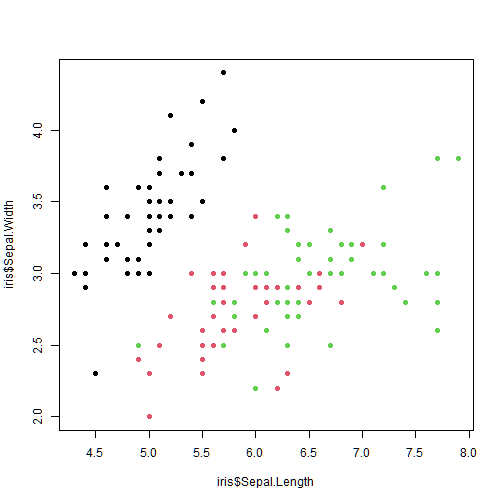
\includegraphics{article_files/figure-latex/code-1} 

}

\caption{The automatic numbering of this figure will only work if it includes a figure caption, user beware!}\label{fig:code}
\end{figure}

Here is an example of an abbreviation where I use the
\texttt{\textless{}abbr\textgreater{}} html tag BT. In the future there
may be a pandoc solution to abbreviation management, however HTML is the
way to go for now.

\hypertarget{understanding-the-method-to-the-madness}{%
\section{Understanding the method to the
madness}\label{understanding-the-method-to-the-madness}}

Need formulas? Here's some \texttt{mathjax} notation:

\[
\beta = \sum^{1 - k}\frac{\delta D}{\sum\frac{\Delta \gamma A}{X-i}}
\]

\hypertarget{adding-tables}{%
\subsection{Adding Tables}\label{adding-tables}}

You can easily add tables to this document like so, and you can also
reference them like a figure, Table @ref(tab:atable):

\begin{longtable}[]{@{}ccccc@{}}
\caption{A caption for the table.}\tabularnewline
\toprule
Sepal L & Sepal W & Petal L & Petal W & Species \\
\midrule
\endfirsthead
\toprule
Sepal L & Sepal W & Petal L & Petal W & Species \\
\midrule
\endhead
5.1 & 3.5 & 1.4 & 0.2 & setosa \\
4.9 & 3.0 & 1.4 & 0.2 & setosa \\
4.7 & 3.2 & 1.3 & 0.2 & setosa \\
4.6 & 3.1 & 1.5 & 0.2 & setosa \\
\bottomrule
\end{longtable}

\hypertarget{the-final-chapter-to-my-pretend-thesis}{%
\section{The final chapter to my pretend
thesis}\label{the-final-chapter-to-my-pretend-thesis}}

There are still a few features that would be nice to implement in the
future for this template. For instance:

\begin{enumerate}
\def\labelenumi{\arabic{enumi}.}
\item
  It would be great to have the ability to use the
  \href{https://github.com/noamross/redoc}{\{redoc\}} package to help
  those who have the ever dreaded ``USE WORD ONLY'' supervisors.
\item
  It would also be great to have the ability to generate a
  \emph{Reference} section for each \emph{Chapter} for those who are
  writing in the ``integrated article'' format.
\item
  Along with that, it would be great to pull the YAML data from a child
  .Rmd file and use it as a way to add the Chapter titles and any other
  subsequent information (for example a thesis chapter can often
  actually be a full manuscript and or published paper which would need
  to have all authors listed for that chapter specifically as well as
  the journal publication information/ citation data).
\end{enumerate}

\hypertarget{references}{%
\section*{References}\label{references}}
\addcontentsline{toc}{section}{References}

\hypertarget{refs}{}
\begin{CSLReferences}{1}{0}
\leavevmode\vadjust pre{\hypertarget{ref-R-knitr}{}}%
Xie, Yihui. 2021. \emph{Knitr: A General-Purpose Package for Dynamic
Report Generation in r}. \url{https://yihui.org/knitr/}.

\end{CSLReferences}

\hypertarget{appendix-i}{%
\section*{APPENDIX I}\label{appendix-i}}
\addcontentsline{toc}{section}{APPENDIX I}

\begin{longtable}[]{@{}ccccc@{}}
\toprule
Sepal.Length & Sepal.Width & Petal.Length & Petal.Width & Species \\
\midrule
\endhead
5.1 & 3.5 & 1.4 & 0.2 & setosa \\
4.9 & 3.0 & 1.4 & 0.2 & setosa \\
4.7 & 3.2 & 1.3 & 0.2 & setosa \\
4.6 & 3.1 & 1.5 & 0.2 & setosa \\
5.0 & 3.6 & 1.4 & 0.2 & setosa \\
5.4 & 3.9 & 1.7 & 0.4 & setosa \\
4.6 & 3.4 & 1.4 & 0.3 & setosa \\
5.0 & 3.4 & 1.5 & 0.2 & setosa \\
4.4 & 2.9 & 1.4 & 0.2 & setosa \\
4.9 & 3.1 & 1.5 & 0.1 & setosa \\
\bottomrule
\end{longtable}

\end{document}
